\section{拉普拉斯变换应用——求解微分方程}

由于拉普拉斯变换的时域的微分性质,LT特别适用于求解微分方程,这给求解系统输出带来方便。

本节要点:
\begin{itemize}
    \item 掌握通过LT求解系统微分方程。
\end{itemize}

%============================================================
\subsection{求解系统微分方程}

用LT求解微分方程步骤:
\begin{enumerate}
    \item 写出系统微分方程。
    \item 两边分别求LT,得到对应的拉普拉斯变换形式。
    \item 求信号的LT,带入得到输出的拉普拉斯变换。
    \item 求iLT,得到输出。
\end{enumerate}

~

若LTI系统有一阶微分方程
\[
\frac{dy\left( t \right)}{dt}+Py\left( t \right) =Qx\left( t \right)
\]
两边LT,得到:
\begin{align*}
&sY\left( s \right) -y\left( 0^- \right) +PY\left( s \right) =QX\left( s \right) \\
&Y\left( s \right) =\frac{1}{s+P}y\left( 0^- \right) +\frac{Q}{s+P}X\left( s \right)
\end{align*}
称为{\bf 系统的复频域表达式}。
输出由初始能量和对输入的响应组成。
特别地,当系统无初始能量时($y\left( 0^- \right) =0$),有:
\[
Y\left( s \right) =\frac{Q}{s+P}X\left( s \right)
\]
令$H\left( s \right) =\frac{Q}{s+P}$,称为{\bf 系统的传递函数}(transfer function)。

若LTI系统有二阶微分方程
\[
\frac{d^2y\left( t \right)}{dt^2}+P_1\frac{dy\left( t \right)}{dt}+P_0y\left( t \right) =Q_1\frac{dx\left( t \right)}{dt}+Q_0x\left( t \right)
\]
两边LT,且由于$x\left( t \right) =0,t<0$,得到:
\[
Y\left( s \right) =\frac{sy\left( 0^- \right) +y'\left( 0^- \right) +P_1y\left( 0^- \right)}{s^2+P_1s+P_0}+\frac{Q_1sX\left( s \right) +Q_0X\left( s \right)}{s^2+P_1s+P_0}
\]
特别地,系统无初始储能时有
\[
Y\left( s \right) =\frac{Q_1s+Q_0}{s^2+P_1s+P_0}X\left( s \right)
\]
称$H\left( s \right) =\frac{Q_1s+Q_0}{s^2+P_1s+P_0}$为{\bf 二阶系统的传递函数}。

更一般地,若LTI系统是n阶微分方程
\[
y^{\left( n \right)}\left( t \right) +\sum_{i=0}^{n-1}{A_iy^{\left( i \right)}\left( t \right)}=\sum_{i=0}^m{B_ix^{\left( i \right)}\left( t \right)}
\]
系统无初始储能时,传递函数为
\[
H\left( s \right) =\frac{B_ms^m+\cdots +B_1s+B_0}{s^n+A_{n-1}s^{n-1}+\cdots +A_1s+A_0}
\]

%============================================================
\subsection{例}

\begin{example}
还是以RC电路为例,假设电容有初始储能$y\left( 0^- \right) $,输入为$x\left( t \right) =u\left( t \right) $,分析输出。
\begin{figure}[h]
\centering
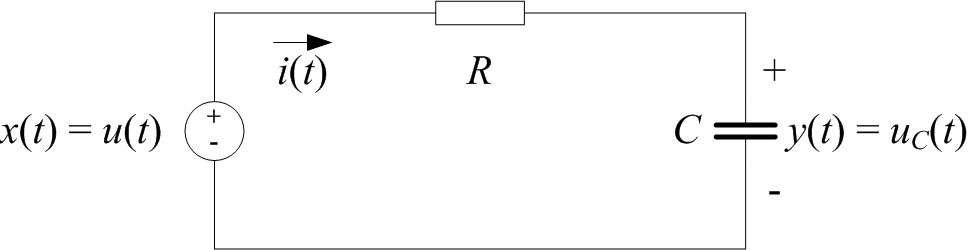
\includegraphics[height=2cm]{1.5.1-1.png}
\end{figure}
\end{example}

系统的微分方程为:
\[
\frac{dy\left( t \right)}{dt}+\frac{1}{RC}y\left( t \right) =\frac{1}{RC}x\left( t \right)
\]
复频域表达式:
\begin{align*}
Y\left( s \right) &=\frac{y\left( 0^- \right)}{s+\left( 1/RC \right)}+\frac{\left( 1/RC \right)}{s+\left( 1/RC \right)}X\left( s \right) \\
&=\frac{y\left( 0^- \right)}{s+\left( 1/RC \right)}+\frac{\left( 1/RC \right)}{s+\left( 1/RC \right)}\cdot \frac{1}{s} \\
&=\frac{y\left( 0^- \right)}{s+\left( 1/RC \right)}+\frac{1}{s}-\frac{1}{s+\left( 1/RC \right)}
\end{align*}
iLT后得到:
\[
y\left( t \right) =y\left( 0^- \right) e^{-\left( 1/RC \right) t}+1-e^{-\left( 1/RC \right) t}
\]
若系统无初始储能,则$y\left( t \right) =1-e^{-\left( 1/RC \right) t}$。




